\chapter{A kész alkalmazás bemutatása}

Az alkalmazás forráskódja elérhető a \url{https://github.com/CptNero/SlimShady} oldalon.

\section{Az alkalmazás fordítása}

\subsection{Függőségek}
Az alkalmazás fordítása előtt a felhasználónak be kell szerezni a GLEW\footnote{\url{https://github.com/nigels-com/glew}} és GLFW3\footnote{\url{https://github.com/glfw/glfw}} könyvtárakat, mint függőségek.

Windows rendszereken ajánlott az előrefordított binárisokat beszerezni, majd elhelyezni őket a Dependencies mappában és a mellékelt CMAKE fájlokat használni a fordítás során.

Linux rendszereken a konyvtárakat magunknak kell telepíteni, majd a CMAKE scriptben a \mintinline{cmake}{find_packages()} paranccsal megkeresni.

A projekt mindkét rendszerhez külön CMAKE build scriptet tartalmaz és a használt header only könyvtárak pedig a Vendor mappában találhatóak.

\newpage
A használt könyvtárak listája:
\begin{itemize}
    \item imgui\footnote{\url{https://github.com/ocornut/imgui}}
    \item imfilebrowser\footnote{\url{https://github.com/AirGuanZ/imgui-filebrowser}}
    \item ImGuiColorTextEdit\footnote{\url{https://github.com/BalazsJako/ImGuiColorTextEdit}}
    \item GLM\footnote{\url{https://github.com/g-truc/glm}}
    \item stb\_image/stb\_image\_write\footnote{\url{https://github.com/nothings/stb}}
    \item Cereal\footnote{\url{https://uscilab.github.io/cereal/}}
    \item date\footnote{\url{https://github.com/HowardHinnant/date}}
\end{itemize}

\subsection{Fordítás}
Az alkalmazás a következő parancsokkal fordítható:
\begin{minted}{cpp}
cmake ~Slimshady
cmake --build ~Slimshady/build/bin
\end{minted}

Az alkalmazás könyvtár struktúrája a \ref{fig:dirtree} ábrán látható:

\begin{figure}[hbt!]
    \centering
    \resizebox{\textwidth}{!}{
    \begin{forest}
    forked edges,
[SlimShady
    [executable]
    [Resources
        [VertexShaders
            [triangle\_Vertex.shader]
        ]
        [FragmentShaders
            [triangle\_Fragment.shader]
        ]
        [Attributes
            [triangle.atrb]
        ]
        [Textures
            [funny\_yellow\_dog.jpg]
            [floppa.png]
            [fumo.bmp]
        ]
        [Tasks
            [triangle.json]
        ]
    ]
]
\end{forest}}
    \caption{Az alkalmazás könyvtár struktúrája}
    \label{fig:dirtree}
\end{figure}

A VertexShaders és a FragmentShaders mappákban helyezkednek el a vertex és a fragmens shaderek forráskódjai. Az attributes mappában helyezkednek el az attribútum fájlok, amik a vertexeket, indexeket és a textúrak elérési útvonalát tartalmazzák. A textures mappában kell elhelyezni a használni kívánt textúrákat. A Tasks mappában pedig az exportált feladatok találhatóak meg JSON formátumban.

\newpage

\section{Az alkalmazás bemutatása}

\subsection{Feladat elkészítése és exportálása}

Amikor a felhasználó elindítja az alkalmazást a \ref{fig:startup} ábra látványával találkozik.

\begin{figure}[hbt!]
    \centering
    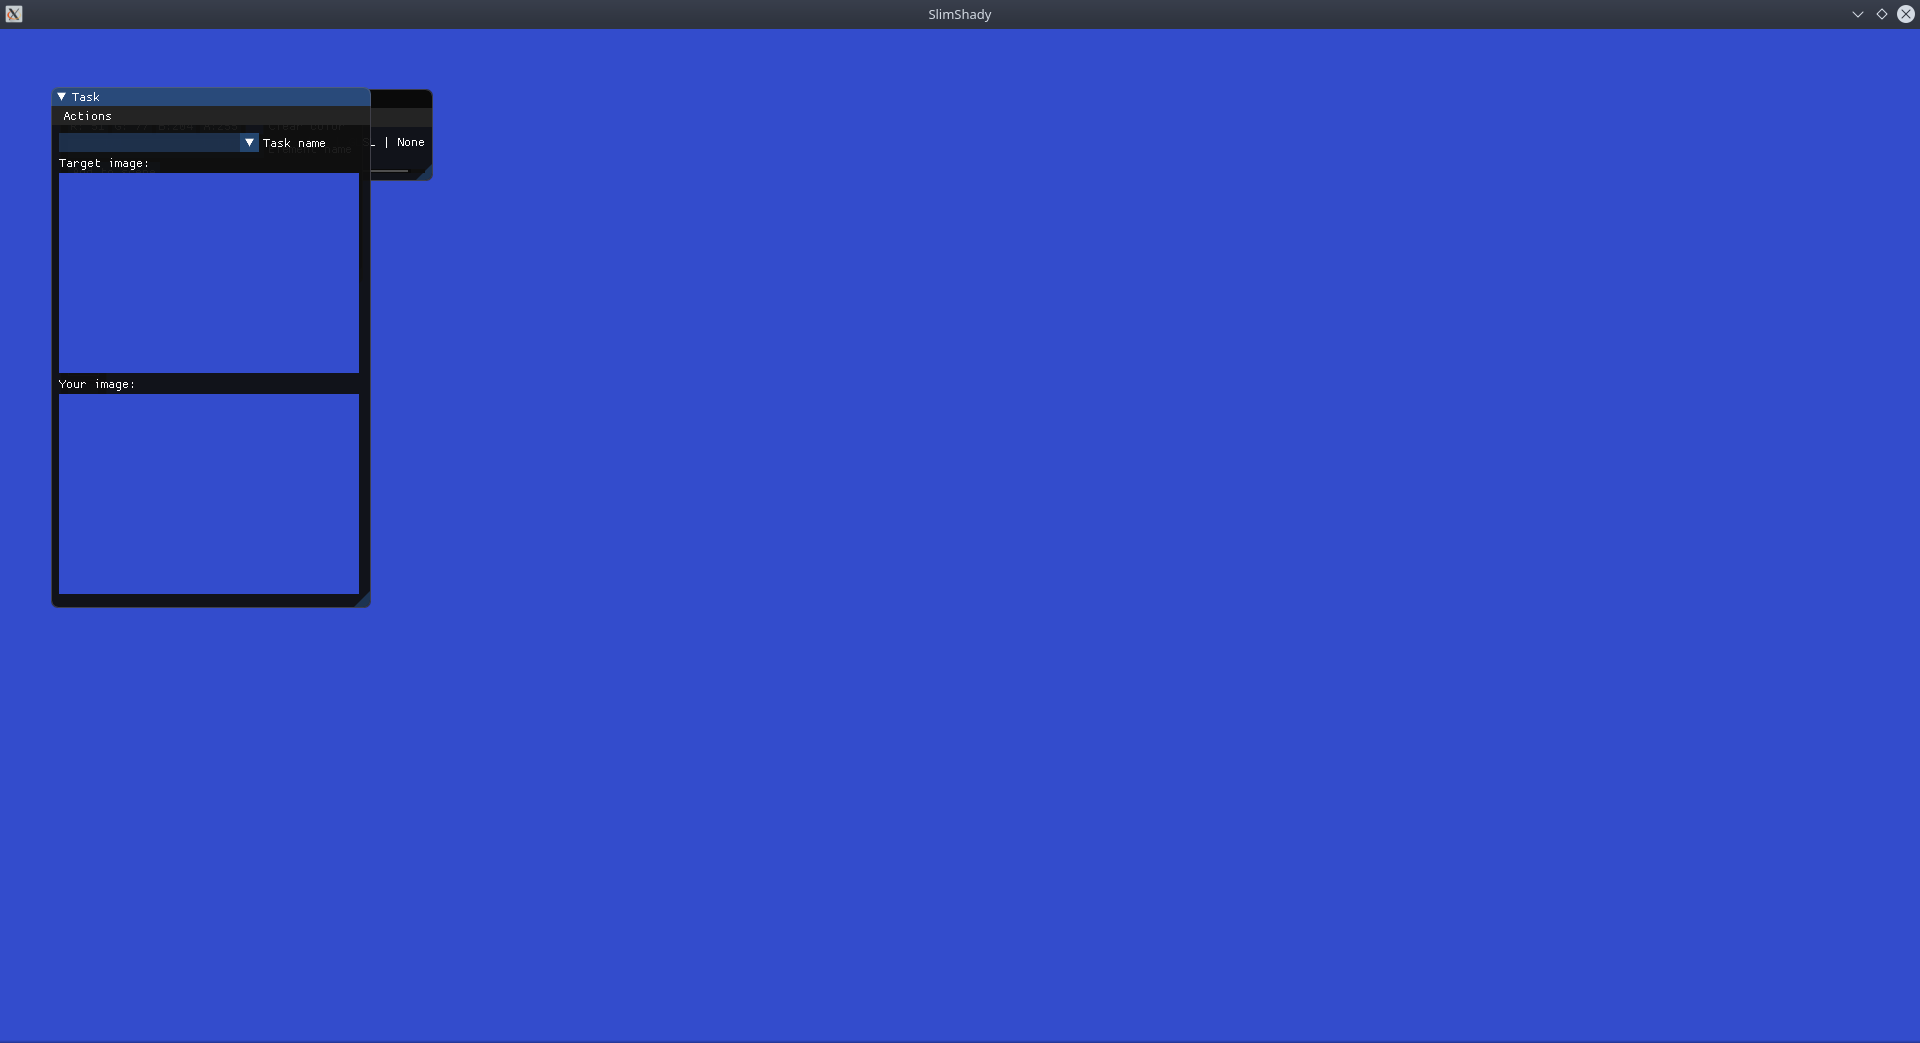
\includegraphics[width=0.75\textwidth,height=\textheight/2,keepaspectratio]
    {resources/Showcase/slimshady_startup.png}
    \caption{Az alkalmazás állapota az első indítás során}
    \label{fig:startup}
\end{figure}

A widgeteket célszerű úgy elrendezni ahogy a felhasználó számára kényelmes, ezt csak egyszer kell megtenni, az alkalmazás a widget pozíciókat megtartja legközelebb is. Egy szépen elrendezett példa látható a \ref{fig:orderedUI} ábrán.

\begin{figure}[hbt!]
    \centering
    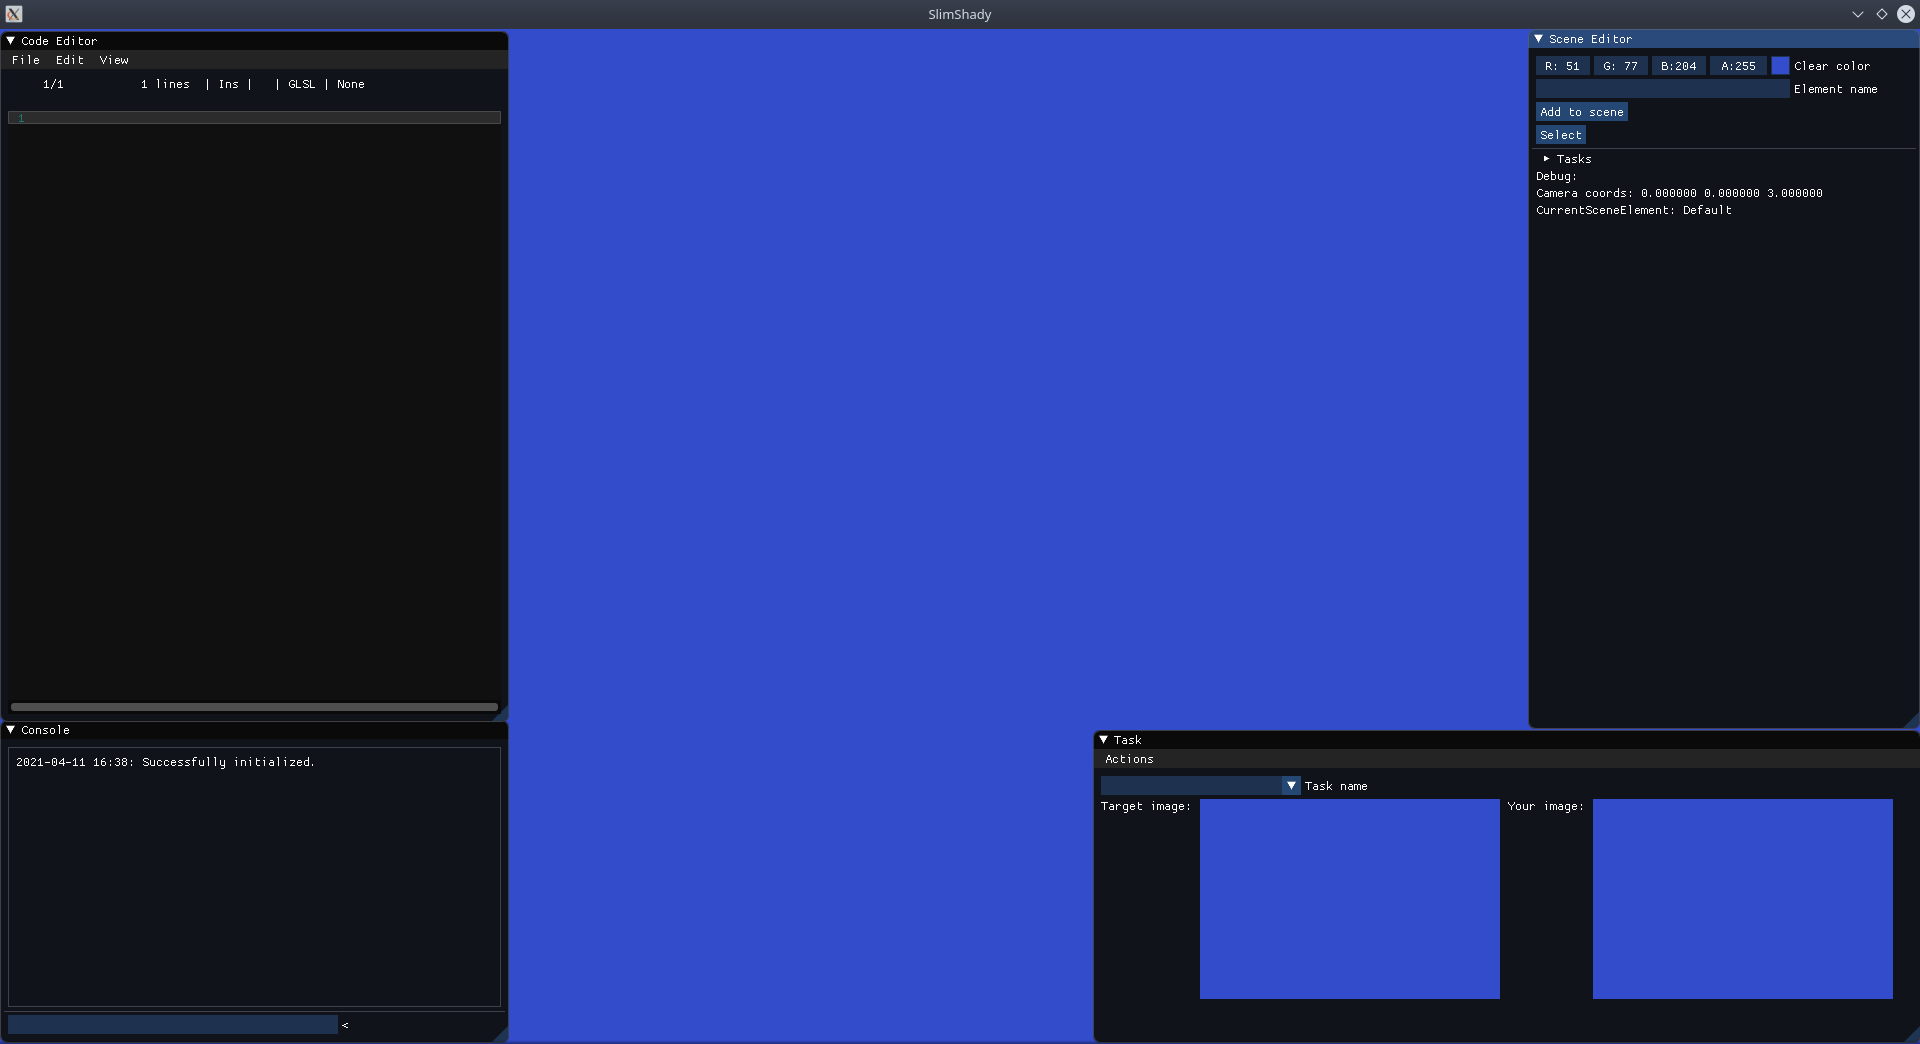
\includegraphics[width=0.75\textwidth,height=\textheight/2,keepaspectratio]
    {resources/Showcase/slimshady_orderedUI.png}
    \caption{Az alkalmazás rendezett UI-al}
    \label{fig:orderedUI}
\end{figure}

\newpage

Hozzunk létre egy új objektumot a \ref{fig:newObject}  ábrán látható \verb|SceneEditor| widget segítségével. Az "Element name" mezőben adjunk meg egy nevet az objektumunknak, majd nyomjuk meg az "Add to scene" gombot.

\begin{figure}[hbt!]
    \centering
    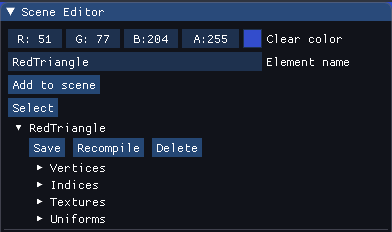
\includegraphics[width=0.5\textwidth,height=\textheight/2,keepaspectratio]
    {resources/Showcase/slimshady_newObject.png}
    \caption{Objektum létrehozása}
    \label{fig:newObject}
\end{figure}

A "vertices" fület lenyitva adhatunk meg új vertexeket és hasonlóan indexeket mint ahogy a \ref{fig:vertices} ábra mutatja. Adjuk meg egy háromszög vertexeit és indexeit, a "Save" gombbal pedig mentsük el őket.

\begin{figure}[hbt!]
    \centering
    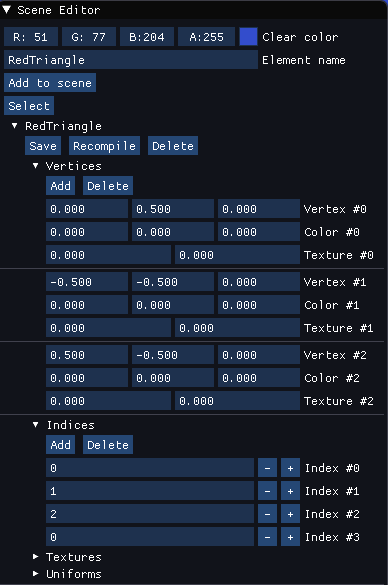
\includegraphics[width=0.4\textwidth,height=\textheight/2,keepaspectratio]
    {resources/Showcase/slimshady_vertices.png}
    \caption{Vertex koordináták beállítása}
    \label{fig:vertices}
\end{figure}

A háromszögünk még nem fog megjelenni, hiszen még nem adtuk meg a vertex és fragmens shadereket. Nyissuk meg az objektumunk vertex shader fájlját a szövegszerkesztőben, melyet a "File" fül alatt az "Open Vertex shaders" opcióval tehetünk meg. A \ref{fig:filebrowser} ábrán látható \verb|FileBrowser| widget jelenik meg előttünk, ahonnan válasszuk ki a vertex shader fájlunkat.

\begin{figure}[hbt!]
    \centering
    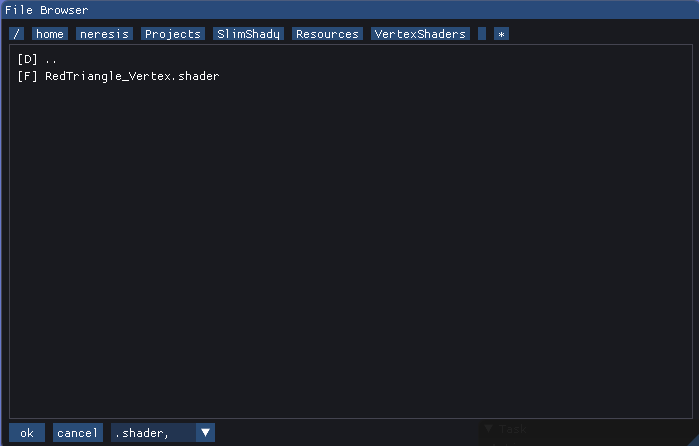
\includegraphics[width=0.75\textwidth,height=\textheight/2,keepaspectratio]
    {resources/Showcase/slimshady_filebrowser.png}
    \caption{Fájl böngésző}
    \label{fig:filebrowser}
\end{figure}

A fájlt kiválasztva a shader kód jelenik meg előttünk a szövegszerkesztőben melyet kedvünkre szerkeszthetünk. 

\subparagraph*{A szerkesztő rendelkezeik pár kényelmi funkcióval:}
\begin{itemize}
    \item Sorok számozása
    \item Tabulálások jelzése
    \item Szintaxis kiemelés
    \item Jelenleg megnyitott fájl elérési utvonalának jelzése
    \item Szöveg statisztika
    \item Többféle szín paletta
\end{itemize}

A kódszerkesztő widget a \ref{fig:vertexcode} ábrán látható.

\begin{figure}
    \centering
    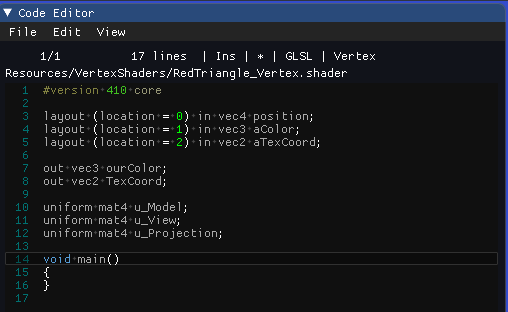
\includegraphics[width=0.75\textwidth,height=\textheight/2,keepaspectratio]
    {resources/Showcase/slimshady_vertexcode.png}
    \caption{Sablon vertex forráskód}
    \label{fig:vertexcode}
\end{figure}

\newpage

Szerkesszük meg úgy a kódot, hogy a vertex pozíciókat a model, nézet és projekciós mátrixokkal beszorozva értékül adjuk mint ahogy a \ref{fig:vertexdone} ábrán láthatjuk, majd a "File" tab alatt a "Save" opcióval mentsük el a fájlt.

\begin{figure}[hbt!]
    \centering
    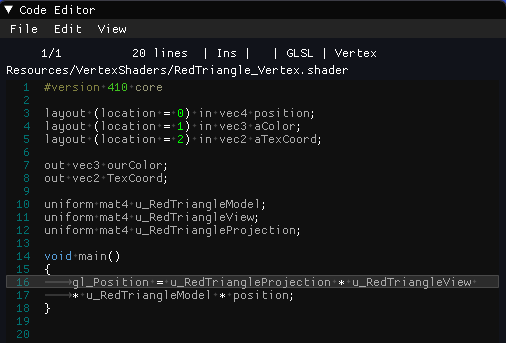
\includegraphics[width=0.75\textwidth,height=\textheight/2,keepaspectratio]
    {resources/Showcase/slimshady_vertexcodeDone.png}
    \caption{Kész vertex forráskód}
    \label{fig:vertexdone}
\end{figure}

Hasonló módon nyissuk meg a fragmens shaderünket és a \verb|FragColor| változót állítsuk be úgy, hogy a háromszögünket pirosra színezzük, szemléltetve a \ref{fig:fragment} ábra által. 

\begin{figure}[hbt!]
    \centering
    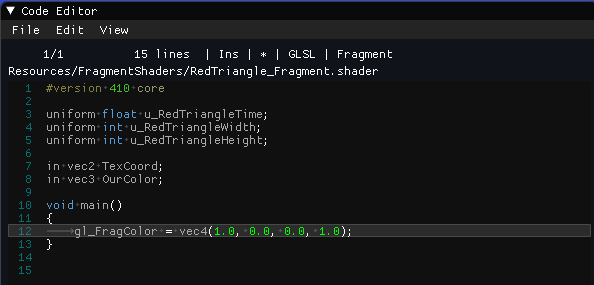
\includegraphics[width=0.75\textwidth,height=\textheight/2,keepaspectratio]
    {resources/Showcase/slimshady_fragment.png}
    \caption{Fragmens forráskód}
    \label{fig:fragment}
\end{figure}

Mentsük el a módosításokat és a \verb|SceneEditor| widgeten nyomjuk meg a "Recompile" gombot. Most már sikeresen megjelenik a piros háromszögünk mint ahogy a \ref{fig:red_triangle} ábrán látható.

\begin{figure}[hbt!]
    \centering
    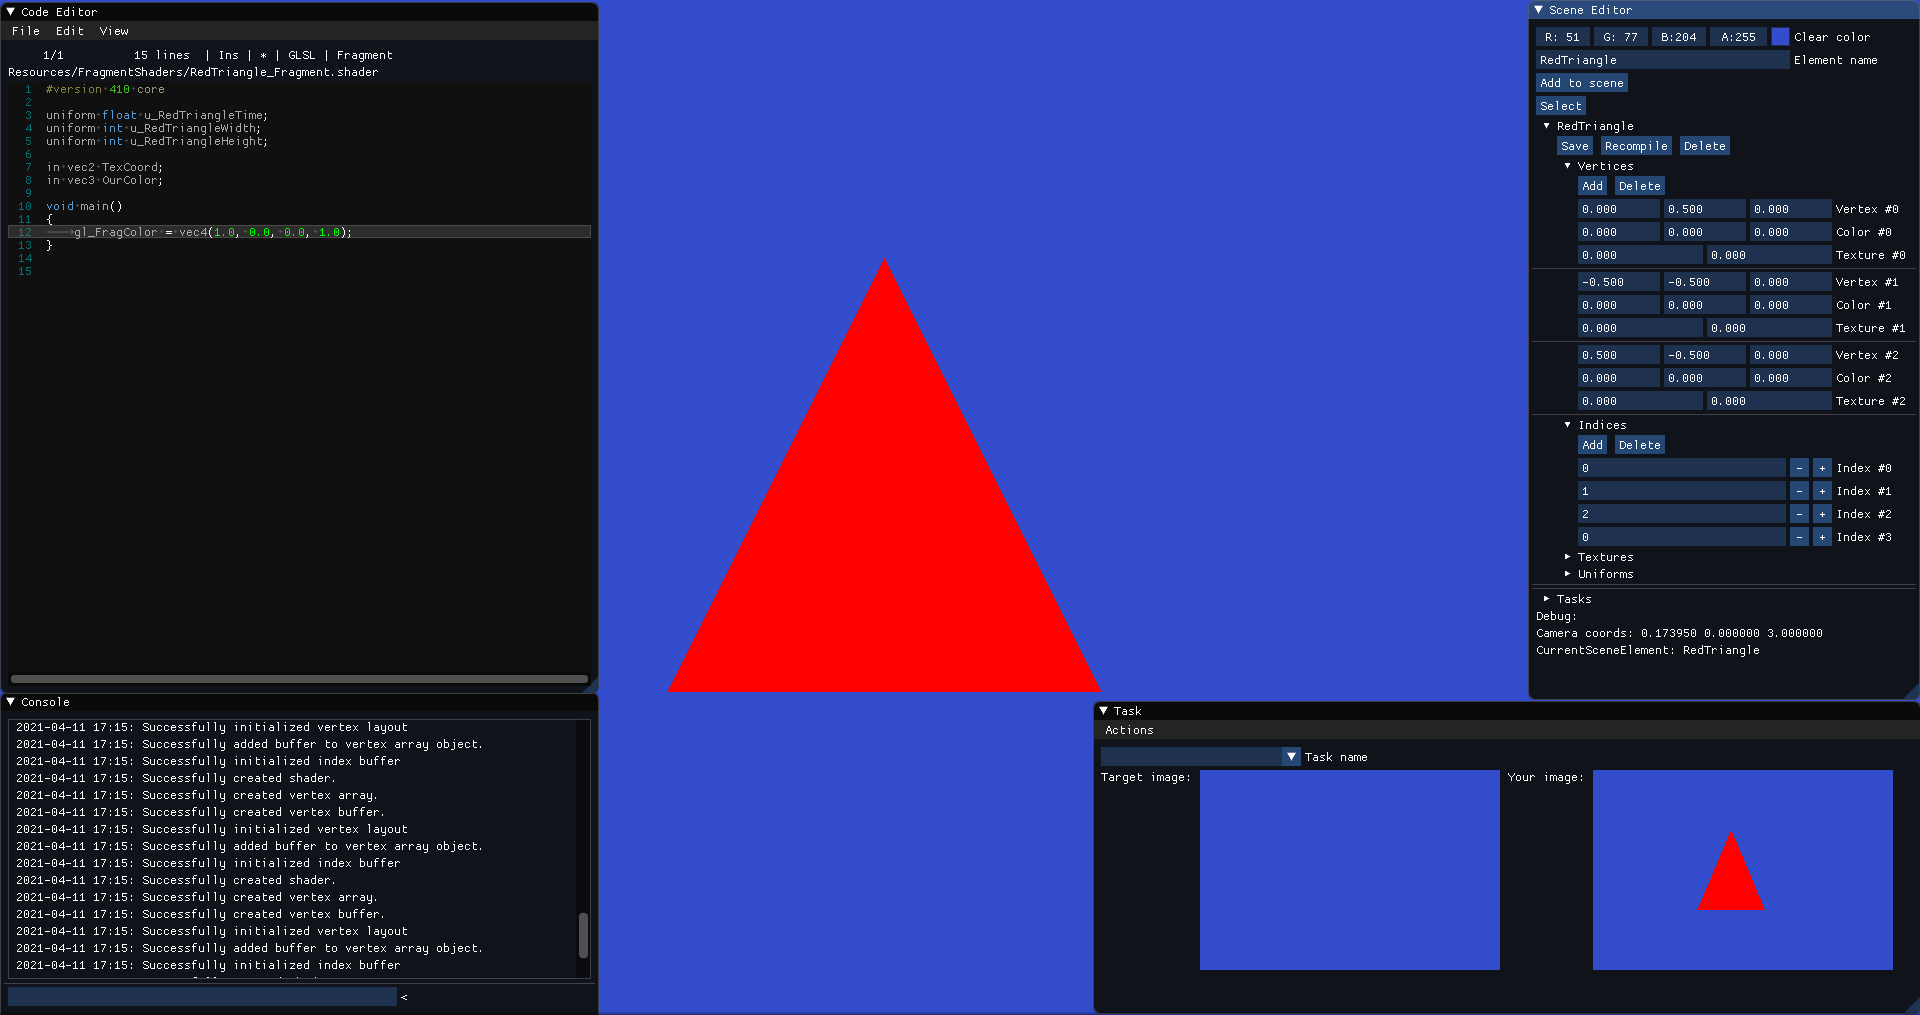
\includegraphics[width=0.75\textwidth,height=\textheight/2,keepaspectratio]
    {resources/Showcase/slimshady_renderedTriangle.png}
    \caption{A kész piros háromszög}
    \label{fig:red_triangle}
\end{figure}

A kész objektumot pedig a \ref{fig:task_export} ábrán látható \verb"Task" widgeten lévő "Actions" fül alatti "Export task" opcióval exportálhatjuk.

\begin{figure}[hbt!]
    \centering
    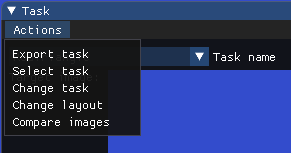
\includegraphics[width=0.35\textwidth,height=\textheight/2,keepaspectratio]
    {resources/Showcase/slimshady_export.png}
    \caption{Feladat exportálása}
    \label{fig:task_export}
\end{figure}


\subsection{Feladat betöltése}

Töltsünk be az előbb exportált feladatot, a \verb"Task" widgeten található "Actions" fül alatt navigáljunk a "Select task" opcióra, válasszuk ki a RedTriangle.json nevű fájlt, majd ugyanitt menjünk rá a "Change task" opcióra. Ezzel már sikeresen be is töltöttünk egy feladatot mint ahogy a \ref{fig:taskwidget} ábrán látható. Egy feladat betöltésekor létrejön egy objektum a megfelelő vertexekkel, indexekkel és textúrákkal, a felhasználónak csak a shader forráskódokat kell megírnia. Nekünk már ez kész van, így csak az eredményeket kell összehasonlítani.

\begin{figure}[hbt!]
    \centering
    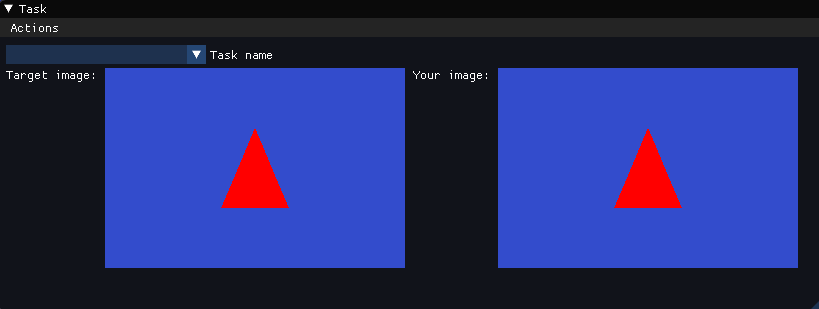
\includegraphics[width=0.75\textwidth,height=\textheight/2,keepaspectratio]
    {resources/Showcase/slimshady_taskwidget.png}
    \caption{Betöltött feladat}
    \label{fig:taskwidget}
\end{figure}

\subsection{Kép összehasonlítás}

Az "Actions" fül alatt válasszuk a "Compare images" opciót, majd az eredmény a \ref{fig:console} ábrán szemléltetett \verb|Console| widgeten jelenik majd meg.

\begin{figure}[hbt!]
    \centering
    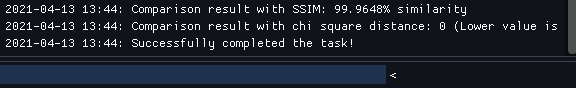
\includegraphics[width=\textwidth,height=\textheight,keepaspectratio]
    {resources/Showcase/slimshady_comparisonresult.png}
    \caption{Összehasonlítás eredménye}
    \label{fig:console}
\end{figure}

A feladat akkor számít sikeresnek, ha az SSIM szerint a képek legalább hetven százalékban hasonlítanak vagy a CSD nyolc tizednél kissebb értéket ad vissza.

Módosítsunk a képünkön úgy, hogy az egy négyzet legyen, amire rárajzolunk egy textúrát.
Először is vegyünk fel még egy vertexet, állítsuk be a textúra koordinátáknál a negyedik vertexet és igazítsuk úgy az indexeket, hogy a negyedik vertexet is felhasználv egy négyzetet rajzoljunk. A beállított értékek a \ref{fig:modifiedvertices} ábrán látható.

A \verb|Scene editor| widgeten a "Select" gombra kattintva választhatunk ki textúrát, amit a Textures fül alatt az "Add" gombbal adhatunk hozzá az objektumunkhoz.

\begin{figure}[hbt!]
    \centering
    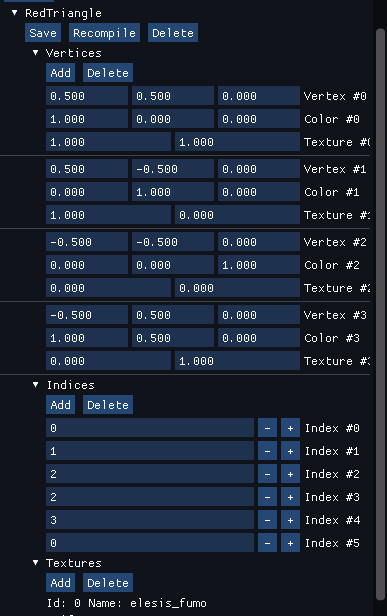
\includegraphics[width=\textwidth/2,height=\textheight/2,keepaspectratio]
    {resources/Showcase/slimshady_modifiedVertices.png}
    \caption{Textúra koordináták beállítása}
    \label{fig:modifiedvertices}
\end{figure}

\newpage

A vertex shaderben pedig adjuk értékül az \verb|OurColor| és a \verb|TexCoord| változóknak a \verb|aColor| és a \verb|aTexCoord| értékeit. Amik azok a koordináták lesznek amiket a \verb|SceneEditor| widgetben adtunk meg. A kész vertex shader a \ref{fig:vertexmodified} ábrán látható.

\begin{figure}[hbt!]
    \centering
    \includegraphics[width=0.75\textwidth,height=\textheight/2,keepaspectratio]
    {resources/Showcase/slimshady_VertexTextureModification.png}
    \caption{Textúra koordináták átadása a vertex shaderben}
    \label{fig:vertexmodified}
\end{figure}

A fragmens shaderben pedig vegyünk fel egy \verb|Sampler2D|-t uniformot a textúránknak, aminek a neve legyen "u\_\{ObjektumNév\}Texture\{Id\}, itt az "ObjektumNév" a shaderhez tartozó objektum neve az "Id" pedig a textúra azonosítója. A samplert állítsuk be textúrának. Ezt a texture függvénnyel tehetjük meg, ami paraméterül vár egy samplert és a textúra koordinátákat, melyeket az \verb|in| változókból kapunk meg a vertex shaderen keresztül. A már textúrát rajzoló fragmens shadert a \ref{fig:settexture} ábrán láthatjuk.

\begin{figure}[hbt!]
    \centering
    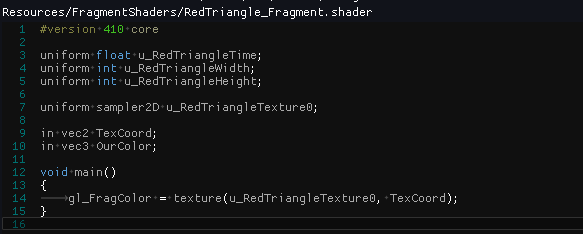
\includegraphics[width=0.75\textwidth,height=\textheight/2,keepaspectratio]
    {resources/Showcase/slimshady_fragmentTexture.png}
    \caption{Textúra beállítása fragmens shaderben}
    \label{fig:settexture}
\end{figure}

Mentsük el a shader forráskódokat és az attribútomkat, majd a "Recompile" gommbal fordítsuk újra az objektumot. Szintén töltsünk be egy másik feladatot is.


\begin{figure}[hbt!]
    \centering
    \includegraphics[width=\textwidth,height=\textheight,keepaspectratio]
    {resources/Showcase/slimshady_badComparison.png}
    \caption{Két különböző kép összehasonlítása}
    \label{fig:badcomparison}
\end{figure}

A \ref{fig:badcomparison} ábrán láthatóan a kettő kép különböző, nézzük meg, hogy a képösszehasonlító funkció szerint is így van-e.

\begin{figure}[hbt!]
    \centering
    \includegraphics[width=\textwidth,height=\textheight,keepaspectratio]
    {resources/Showcase/slimshady_badComparisonResult.png}
    \caption{Különböző képek összehasonlításának eredménye}
    \label{fig:badcomparisonresult}
\end{figure}

A \ref{fig:badcomparisonresult} ábrán lájuk, hogy a két kép egyik metrika szerint sem egyezik, így mondhatjuk azt, hogy a képösszehasonlítás funkció megfelelően működik.

